\section{Problem 2}
\label{part2}
\begin{verbatim}
(extra credit, 3 points)

We know the group split in two different groups.  Suppose the
disagreements in the group were more nuanced -- what would the clubs
look like if they split into groups of 3, 4, and 5?

\end{verbatim}

\subsection{Solution}
\begin{enumerate}
\item This is almost similar to the solution of question 1, the only difference is to get 3, 4 and 5 clusters rather than 2.
\item The initial graph can be seen in figure\ref{b2} and the code can be seen in listing\ref{lst:q2-1}
\item The graphs with 3, 4 and 5 clusters can be seen in figure\ref{d4}, figure\ref{e5}, figure\ref{f6}
\end{enumerate}
\newpage
\subsection{Code Listing}
Here is the Python program for dividing 1 cluster into 3,4,5 clusters consecutively

\lstinputlisting[language=Python,breaklines = true,frame=single,caption={Python code}, label=lst:q2-1,captionpos=b,numbers=left,showspaces=false,showstringspaces=false,basicstyle=\footnotesize]{sam_karate_2.py}
\newpage
\subsection{Results}

\subsubsection{Sample Karate GraphML file given as input to the program}
\begin{figure}[ht]    
    \begin{center}
        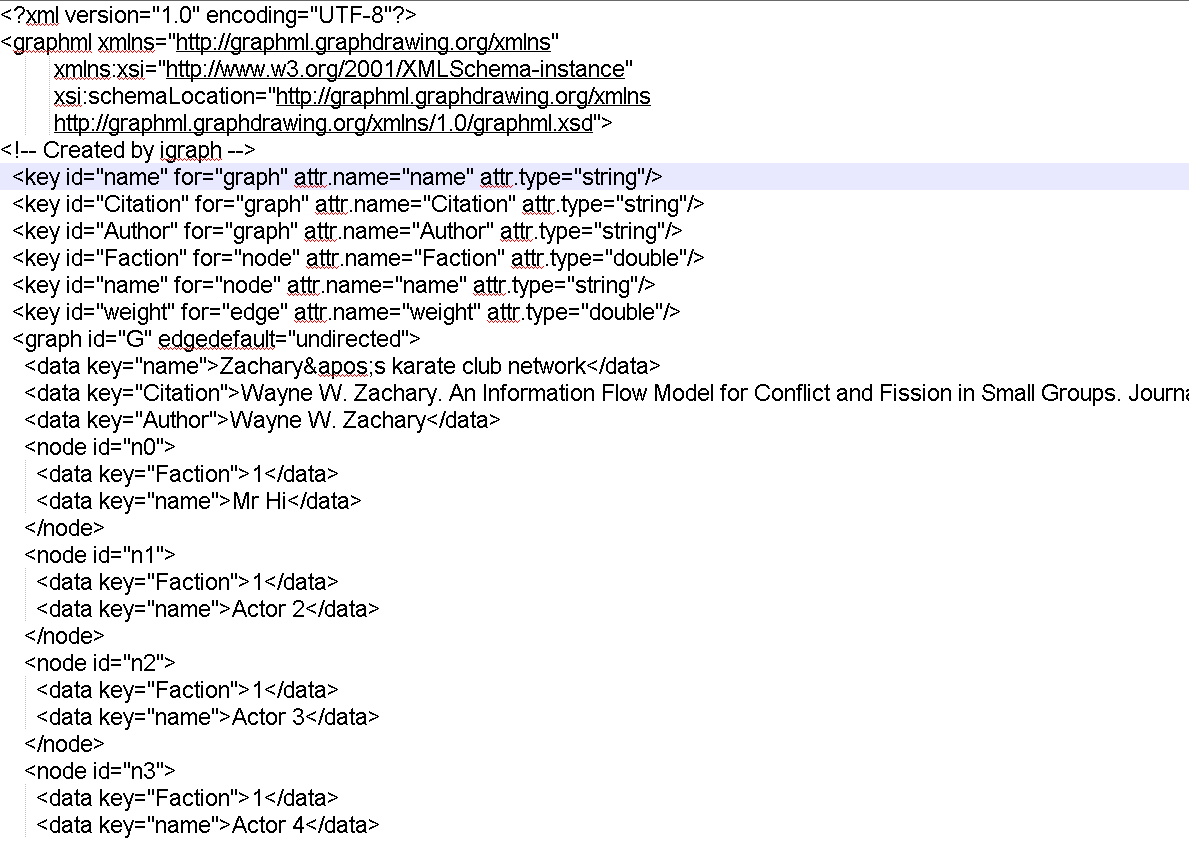
\includegraphics[scale=0.7]{input2.png}
         \caption{Sample GraphML file}
        \label{a1}
    \end{center}
\end{figure}
\newpage
\subsubsection{Graph before splitting into 3/4/5 clusters}
\begin{figure}[ht]    
    \begin{center}
        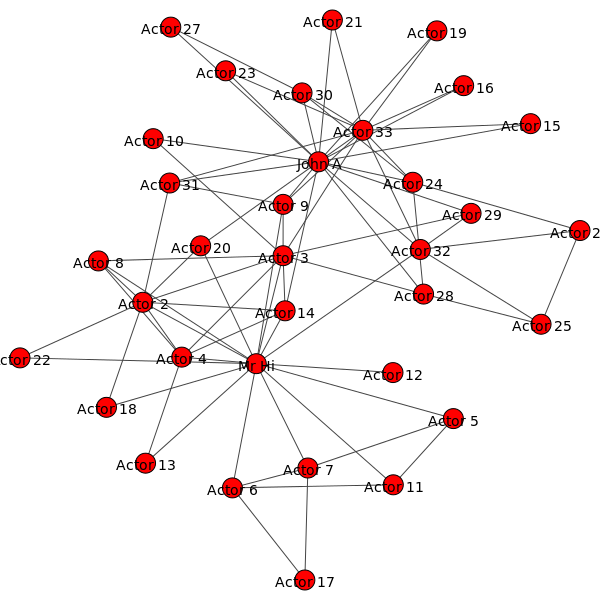
\includegraphics[scale=0.7]{group2.png}
         \caption{Original Graph}
        \label{b2}
    \end{center}
\end{figure}
\newpage

\subsubsection{Command line output of nodes in each cluster and number of edges deleted to get 2 clusters}
\begin{figure}[ht]    
    \begin{center}
        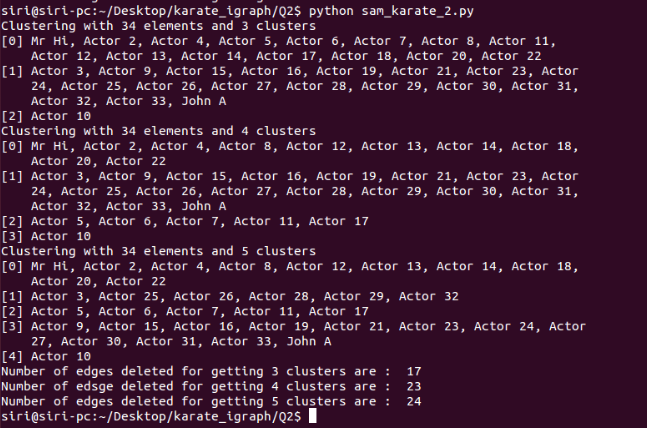
\includegraphics[scale=0.9]{cmd_2.png}
         \caption{Command line output}
        \label{c3}
    \end{center}
\end{figure}
\newpage

\subsubsection{Graph after splitting into 3 clusters}
\begin{figure}[ht]    
    \begin{center}
        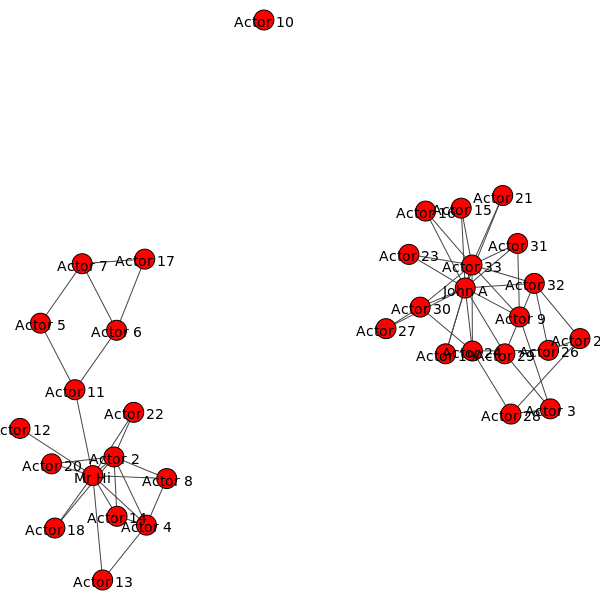
\includegraphics[scale=0.7]{output2.png}
         \caption{3 clusters}
        \label{d4}
    \end{center}
\end{figure}
\newpage

\subsubsection{Graph after splitting into 4 clusters}
\begin{figure}[ht]    
    \begin{center}
        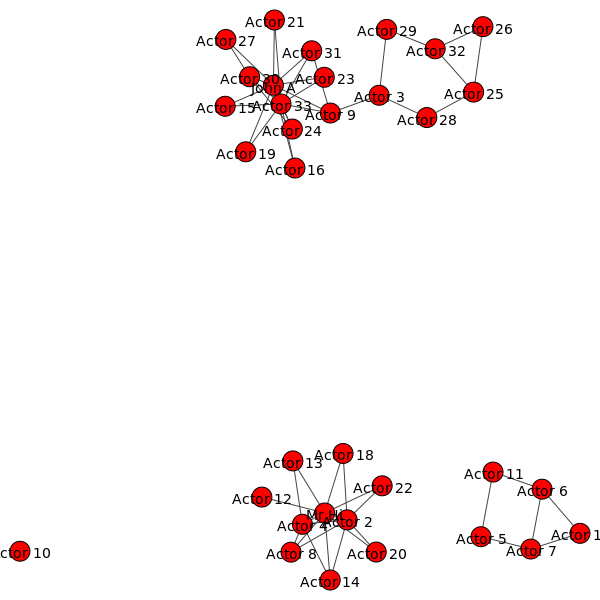
\includegraphics[scale=0.7]{output3.png}
        \caption{4 clusters}
        \label{e5}
    \end{center}
\end{figure}
\newpage
\subsubsection{Graph after splitting into 5 clusters}
\begin{figure}[ht]    
    \begin{center}
        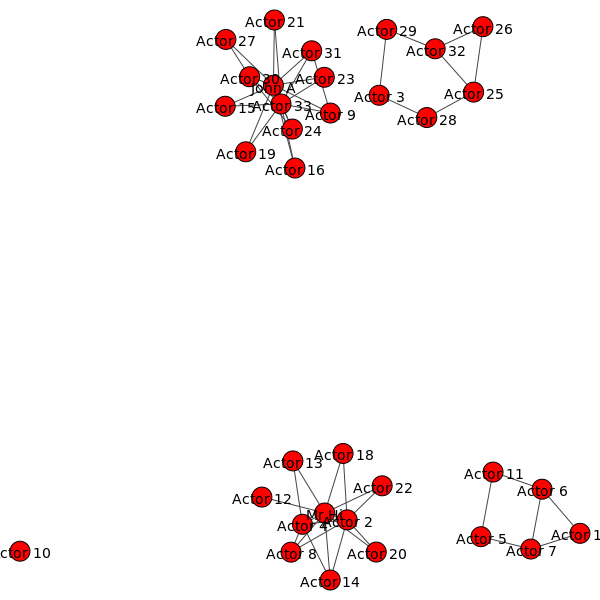
\includegraphics[scale=0.7]{output4.png}
        \caption{5 clusters}
        \label{f6}
    \end{center}
\end{figure}
\newpage
